\chapter{METHODOLOGY}
The broad plan and justification for your research effort are referred to as your methodology. It entails researching the theories and ideas that underpin the procedures employed in your industry in order to create a strategy that is in line with your goals.There are various types of images of ocular diseases. We chose cataracts, glaucoma, pathological myopia, and hypertensive retinopathy to work with. For each model (VGG19, Resnet50, Mobilenetv2), we tested Normal vs. Cataract, Normal vs. Glaucoma, Normal vs. Myopia, and Normal vs. Hypertension. We take 100 epoch for every model. We resize every images 224*224. We also did use some function for time reduction. EarlyStopping class stops training when a monitored metric has stopped improving. ReduceLROnPlateau class reduces learning rate when a metric has stopped improving. Here is the working steps. 
\vspace{5pt}
\begin{figure}[H]
    \centering
    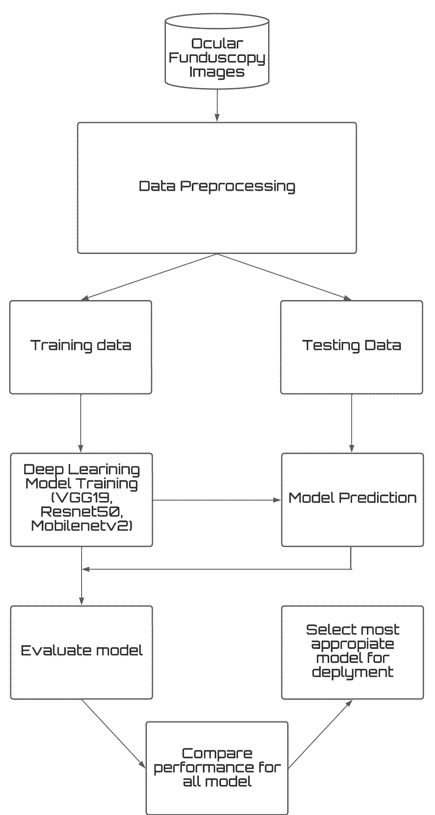
\includegraphics[scale=1]{3.png}
    \caption{Working steps}
    \label{Working steps}
\end{figure}
\section{Classification Using Resnet50}
ResNet50 is a variant of the Resnet model,, which has 48 convolution layers along with 1 MaxPool and 1 Average Pool layer. It has 3.8 x 109 floating point operations. It is a widely used ResNet model, and we have explored the ResNet50 architecture in depth. So as we can see in the resnet 50 architecture contains the following element:
\begin{enumerate}
    \item A convolution with a kernel size of 7 * 7 and 64 different kernels all with a stride of size 2 giving us 1 layer.
    \item Next we see max pooling with also a stride size of 2.
    \item In the next convolution there is a 1 * 1,64 kernel following this a 3 * 3,64 kernel and at last a 1 * 1,256 kernel, These three layers are repeated in total 3 time so giving us 9 layers in this step.
    \item Next we see kernel of 1 * 1,128 after that a kernel of 3 * 3,128 and at last a kernel of 1 * 1,512 this step was repeated 4 time so giving us 12 layers in this step.
    After that there is a kernal of 1 * 1,256 and two more kernels with 3 * 3,256 and 1 * 1,1024 and this is repeated 6 time giving us a total of 18 layers.
    \item And then again a 1 * 1,512 kernel with two more of 3 * 3,512 and 1 * 1,2048 and this was repeated 3 times giving us a total of 9 layers.
    \item We do a average pool and end it with a fully connected layer containing 1000 nodes and at the end a softmax function so this gives us 1 layer.
\end{enumerate}
\begin{figure}[H]
    \centering
    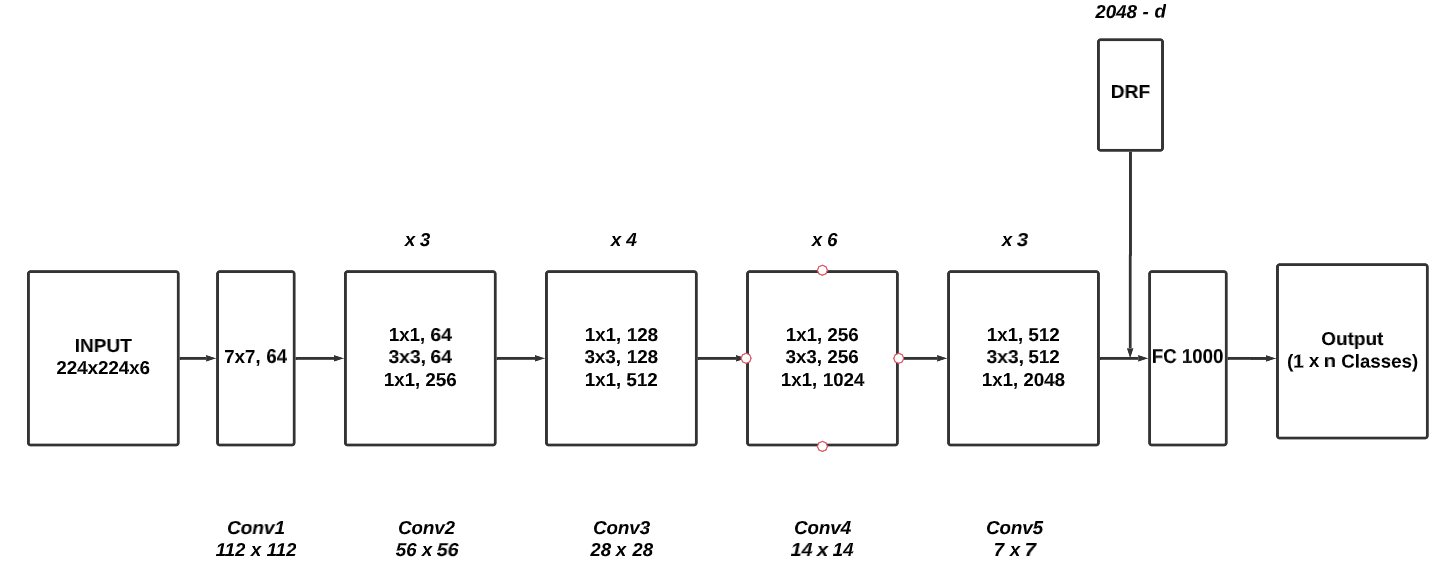
\includegraphics[scale=0.5]{40_Chapter_4/resnet50.png}
    \caption{Resnet50 Architecture}
    \label{Resnet50 Architecture}
\end{figure}
\section{Classification Using VGG19}
A variation of the VGG model called VGG19 has 19 layers in total (16 convolution layers, 3 Fully connected layer, 5 MaxPool layers and 1 SoftMax layer). There are further VGG variations, including VGG11, VGG16, and others. 19.6 billion FLOPs make up VGG19. So as we can see in the VGG19architecture contains the following element:
\begin{enumerate}
    \item A fixed size of (224 * 224) RGB image was given as input to this network which means that the matrix was of shape (224,224,3).
    \item The only preprocessing that was done is that they subtracted the mean RGB value from each pixel, computed over the whole training set.
    \item Used kernels of (3 * 3) size with a stride size of 1 pixel, this enabled them to cover the whole notion of the image.
    \item spatial padding was used to preserve the spatial resolution of the image.
    \item max pooling was performed over a 2 * 2 pixel windows with sride 2.
    \item this was followed by Rectified linear unit(ReLu) to introduce non-linearity to make the model classify better and to improve computational time as the previous models used tanh or sigmoid functions this proved much better than those.
    \item implemented three fully connected layers from which first two were of size 4096 and after that a layer with 1000 channels for 1000-way ILSVRC classification and the final layer is a softmax function.
\end{enumerate}
\begin{figure}[H]
    \centering
    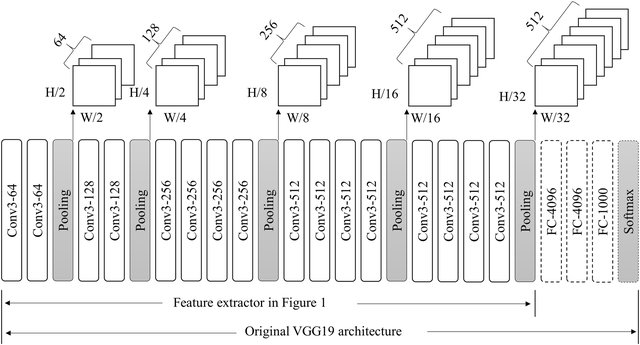
\includegraphics[scale=0.7]{40_Chapter_4/VGG19.jpg}
    \caption{VGG19 Architecture}
    \label{VGG19 Architecture}
\end{figure}
\vspace{5pt}
\section{Classification Using MobilenetV2}
We have explored MobileNet V2 architecture in depth. MobileNet V2 model has 53 convolution layers and 1 AvgPool with nearly 350 GFLOP. It has two main components:
\begin{enumerate}
    \item Bottleneck Residual Block
    \item Inverted Residual Block
\end{enumerate}
There are two types of Convolution layers in MobileNet V2 architecture:
\begin{enumerate}
    \item 1x1 Convolution
    \item 3x3 Depth wise Convolution 
\end{enumerate}
There are three streams and the input shape is 224x224. Our design involves a filter size of 32 for padding, a kernel size of 3, and activation function based on ReLU for the two first layers. The first max pooling layer has a pool size of 2 and strides of 2. The further plain layer combines all of the pooled characteristics into a separate cell. In the end, two thick layers were produced. The activation function for the first layer is ReLU, while the activation function for the least thick layer is softmax. The features are added to the network once they have been pre-processed. A bird's-eye perspective of the structure is shown below.
\begin{figure}[H]
    \centering
    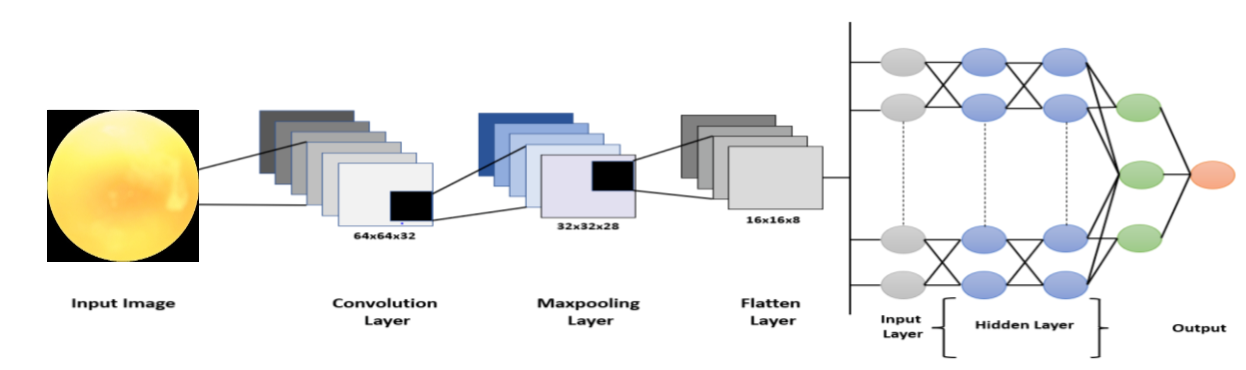
\includegraphics[scale=0.5]{40_Chapter_4/Mb2.png}
    \caption{MobileNetV2 Architecture}
    \label{MobileNetV2 Architecture}
\end{figure}
\vspace{5pt}
\section{Evaluation}
We should be prepared with several assessment metrics to examine the classification algorithm in the event of a classification problem. As follows:
\begin{enumerate}
    \item \textbf{Confusion Matrix:} The classification model's accuracy in classifying instances into distinct groups is summarized in a table called the confusion matrix. The model's anticipated label is on one axis of the confusion matrix, while the actual label is on the other. When comparing several models, we may use the confusion matrix to assess how well each one predicted true positives (TP) and true negatives (TN). We chose a model as our basic model if it accurately predicted TP and TN compared to other models.
\begin{figure}[H]
    \centering
    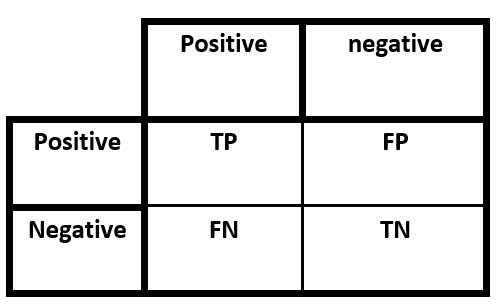
\includegraphics[scale=0.7]{40_Chapter_4/4.png}
    \caption{Confusion Matrix}
    \label{Confusion Matrix}
\end{figure}
TP = True Positive (The total number of images that are
correctly detected to be positive)\\
FP = False Positive (The total number of images that are
predicted to be positive but actually are negative)\\
TN = True Negative (The number of images that are
accurately predicted to be negative)\\
FN = False Negative (The number of images that are
incorrectly predicted to be negative)\\
    \item \textbf{Precision and Recall:} Precision and recall are two metrics used to evaluate classification and retrieval systems' performance. Precision is the percentage of relevant occurrences among all retrieved examples. Recall, also known as sensitivity, is the percentage of recovered instances among all appropriate models. In a perfect classifier, precision and recall are both one. 
\newline
\begin{align*}
Recall = \frac{TP}{TP+FP} 
\\
Precision = \frac{TP}{TP+FP}
\end{align*}
\newline
    \item \textbf{Accuracy:} It is calculated by dividing the total number of correctly categorized instances by the overall number of classified examples. When the importance of each class's prediction error is equal, this measure is crucial. Here, false positives should be addressed more than false negatives.
\newline
\begin{align*}
Accuracy = \frac{TP+tn}{TP+TN+FP+FN} 
\end{align*}
\newline
    \item \textbf{F1 score:} A weighted average of recall and accuracy is the F1 score. False positive and false negative results can occur in accuracy and recall, as is well known, thus both are taken into account. In most cases, the F1 score is more helpful than accuracy, particularly if your class is distributed unevenly. When false positives and false negatives cost about the same, accuracy performs best. It is preferable to include both Precision and Recall if the costs of false positives and false negatives are significantly different.
\newline
\begin{align*}
F1 Score = \frac{2*Recall*Precision}{Recall+Precision} 
\end{align*}
\newline
    \item \textbf{Learning Curve:} For algorithms that learn (optimize their internal parameters) gradually over time, like deep learning neural networks, learning curves are frequently employed in machine learning. If maximization is the metric used to measure learning, then higher scores (bigger numbers) signify more learning. Accuracy in categorisation might serve as an example. It is more typical to employ a score that minimizes, like loss or error, where better scores (lower numbers) imply greater learning and a value of 0.0 indicates that the training dataset was learnt properly with no errors. Additionally, a hold-out validation dataset that is separate from the training dataset can be used to test it. An assessment of the validation dataset provides insight into the model's "generalizability."
\end{enumerate}